% This example is meant to be compiled with lualatex or xelatex
% The theme itself also supports pdflatex
\PassOptionsToPackage{unicode}{hyperref}
\documentclass[aspectratio=1610, 12pt]{beamer}

% Load packages you need here
\usepackage[english]{babel}

\usepackage{csquotes}
    
\usepackage{xcolor}
\usepackage{listings}
\usepackage{amsmath}
\usepackage{amssymb}
\usepackage{mathtools}
\usepackage{hyperref}
\usepackage{bookmark}
\usepackage{array}
\usepackage{tikz}
\usetikzlibrary{positioning,shapes,fit}
\usetikzlibrary{calc}
\usetikzlibrary{arrows.meta}
\usepackage{varwidth}


% load the theme after all packages

\usetheme[
  showtotalframes % show total number of frames in the footline
]{tudo}


\lstdefinestyle{cstyle}{
	belowcaptionskip=1\baselineskip,
	breaklines=true,
	frame=single,
	xleftmargin=\parindent,
	language=C,
	escapeinside={(*@}{@*)},
	showstringspaces=false,
	basicstyle=\footnotesize\ttfamily,
	keywordstyle=\bfseries\color{green!40!black},
	commentstyle=\itshape\color{purple!40!black},
	identifierstyle=\color{gray},
	stringstyle=\color{orange},
}
% Put settings here, like
\makeatletter
\newcommand{\thickhline}{%
	\noalign {\ifnum 0=`}\fi \hrule height 1pt
	\futurelet \reserved@a \@xhline
}
\newcolumntype{"}{@{\hskip\tabcolsep\vrule width 1pt\hskip\tabcolsep}}

\definecolor{preload}{RGB}{184, 17, 17} 
\definecolor{mm1}{RGB}{189, 117, 28}
\definecolor{mm2}{RGB}{130, 22, 87}
\definecolor{mm3}{RGB}{15, 112, 57}


\title{TODO Titel}
\author[Diep, Köhler, Naumann]{Jack Diep, Florian Köhler, Yannick Naumann}
\institute[BNN-Training]{Design Your Own CPU - Design of Embedded Systems}
\titlegraphic{\includegraphics[width=0.675\textwidth]{images/tudo-title-2.jpg}}

\setbeamertemplate{section in toc}{%
	{\color{tugreen}\inserttocsectionnumber.}~\inserttocsection}
\setbeamercolor{subsection in toc}{bg=white,fg=structure}
\setbeamertemplate{subsection in toc}{%
	\hspace{1.2em}{\color{tugreen}\rule[0.3ex]{3pt}{3pt}}~\inserttocsubsection\par}



 \begin{document}


\maketitle




\begin{frame}{Content}
\tableofcontents


\end{frame}
\section{Neural Networks}

\section{BNN Design}
\begin{frame}{Binarisation of Linear Layer}
Inhalt...
\end{frame}
\begin{frame}{Activation}
Inhalt...
\end{frame}
\begin{frame}{Batch Norm (BN)}
\begin{itemize}
	\item In NN
	\begin{itemize}
		\item normalize batches 
		\item mean 0
		\item standard derivation 1 
	\end{itemize}
	\item In BNN 
	\begin{itemize}
		\item prevent expolding gradient %TODO graphic
	\end{itemize}
\end{itemize}
\end{frame}
\begin{frame}{Evaluation of last layer}
\begin{columns}
	\column{0.49\textwidth}
	\begin{itemize}
		\item normalisation of activation
		\item decision of the network
	\end{itemize}
	\column{0.49\textwidth}
	\centering
	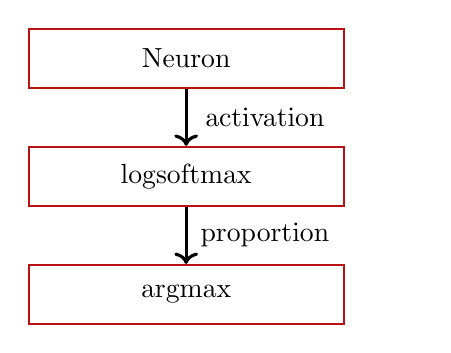
\begin{tikzpicture}[minimum height=0.75cm,minimum width=4cm,line width = 0.25mm]
	\node[rectangle,draw=preload] (neuron) {Neuron};
	\node[rectangle,draw=preload] (softm) at(0,-1.5) {logsoftmax};
	\node[rectangle,draw=preload] (argm) at(0,-3)  {argmax};
	
	\draw [->,line width = 0.4mm] (neuron) -- (softm) node[] at(1,-0.75) {activation};
	\draw [->,line width = 0.4mm] (softm) -- (argm) node[] at(1,-2.25) {proportion};
	\end{tikzpicture}
	
\end{columns}
\end{frame}

\section{BNN Training Analysis}
\begin{frame}
\tableofcontents[currentsection]
\end{frame}
\subsection{Layer Analysis}
\begin{frame}{Effect of Batch Norm}
 	\begin{columns}
 		\column{0.49\textwidth}
 		\begin{itemize}
 			\item 7.4\% improved peak performance
 			\item Less jitter with BN
 			\item Reduced expolding gradient
 		\end{itemize}
 		
 		\column{0.49\textwidth}
 		\centering
 		\includegraphics[scale=0.45]{images/batchnorm_measurement.pdf}
 	\end{columns}
\end{frame}
\begin{frame}{Consequences of linear layer binarisation}


\begin{columns}
	\column{0.49\textwidth}
	\centering
		\begin{tabular}{|c|c|c|}\hline
		Run&binary&normal\\\hline
		1&88.29\%&97.43\%\\\hline
		2&87.32\%&96.98\%\\\hline
		3&87.19\%&97.2\%\\\hline
	\end{tabular}	
	\column{0.49\textwidth}
	\begin{itemize}
		\item TODO
	\end{itemize}
	
\end{columns}


\end{frame}

\subsection{Parameter Analysis}
\begin{frame}{learning rate}
Inhalt...
\end{frame}






\end{document}
